\documentclass[12pt]{article}
 
\usepackage{enumerate}
\usepackage{amsmath,amsthm,amssymb}
\usepackage{mathrsfs} % to use mathscr fonts

\usepackage{epstopdf}
\usepackage{caption,subcaption}
\usepackage{pstricks}
\usepackage{pst-solides3d}
\usepackage{pstricks-add}
\usepackage{graphicx}
\usepackage{pst-tree}
\usepackage{pst-poly}
\usepackage{calc,ifthen}
\usepackage{float}\usepackage{multicol}
\usepackage{multirow}
\usepackage{array}
\usepackage{longtable}
\usepackage{fancyhdr}
\usepackage{algorithmicx,algpseudocode}
\usepackage{changepage}
\usepackage{color}
\usepackage{listings}
\usepackage{fancyvrb}
\usepackage{verbatim,moreverb}
\usepackage{courier}
\lstset{ %
language=C++,               
basicstyle=\footnotesize,
numbers=left,                  
numberstyle=\tiny,     
stepnumber=1,         
numbersep=5pt,         
backgroundcolor=\color{white},  
showspaces=false,               
showstringspaces=false,         
showtabs=false,                 
columns=fullflexible,
frame=single,          
tabsize=2,          
captionpos=b,       
extendedchars=true,
xleftmargin=17pt,
framexleftmargin=17pt,
framexrightmargin=17pt,
framexbottommargin=4pt,
breaklines=true,       
breakatwhitespace=false, 
escapeinside={\%*}{*)}       
}


\newenvironment{block}{\begin{adjustwidth}{1.5cm}{1.5cm}\noindent}{\end{adjustwidth}}
\def\verbatimtabsize{4\relax}
\def\listingoffset{1em}
\def\listinglabel#1{\llap{\tiny\it\the#1}\hskip\listingoffset\relax}
\def\mylisting#1{{\fontsize{10}{11}\selectfont \listinginput[1]{1}{#1}}}
\def\myoutput#1{{\fontsize{9}{9.2}\selectfont\verbatimtabinput{#1}}}


\cfoot{\ \hfill\tiny\sl Draft printed on \today}
 
\title{A Block-Level Encryption Method for Cloud Storage}
\author{Jordan Blocher}

\begin{document}
\maketitle

\section{Introduction}
The solution presented here intends to provide block-level encryption to cloud storage users,
allowing them to manage thier own security without the need to use complicated encryption schemes
based on the file system.

\section{Cloud Storage}
The main challenge of cloud storage is to guarantee integrity, confidentiality and
control over all stored data. 
The cost benefits of cloud storage are so compelling that most turn a blind eye to the security 
shortcomings of this virtualized environment.
Therefore, users should apply security-oriented cloud
storage middleware that, on the one hand, keeps the usage of the cloud simple and fast, and,
on the other hand, enforces the application of strong cryptographic algorithms and protocols in
order to keep private and confidential data from being leaked. 
Stealing data from the cloud is easy, as we can see by \cite{mutch10}. The new data compromisation
methods, known as "Man in the Cloud Attacks" and described in \cite{imperva}, imply that cloud security
is a complex and largely unadressed problem.
Overwhelmingly, current solutions
apply server-side encryption and the user has no control over how the encryption is done and
who has access to the decryption keys. An example of this is the popular cloud storage system 
Dropbox. If the user does have key access control, as in \cite{tresorit}, the cloud
system is only capable of managing encrypted files, which becomes intractable for large data
sets. 
~\\~\\
We make use of block-level encryption techniques in order to construct a method for encryption that is independent of the filesystem. We implement a virtual volume overlaying a series of small encrypted blocks. This allows for the filesystem to be completely independent of the encryption. The size of the blocks allows for rapid synchronization as well as provides an additional level of obsfucation as the storage can be a random array of data blocks, to be reassembled only on the client-side. 

\section{Architecture}

In this section we describe the tools used in order to implement the block-level encrypted storage, and provide some detail as to how the method differs from current implementations using these tools to create encryption schemes. The scheme makes use of the Linux kernel toolkit and core-utils. The encryption scheme presented in this report makes use of the following Linux utilities:
\begin{verbatim}
parted:
\end{verbatim}
A partitioning utility used to prepare the BASE drive for encryption.
\begin{verbatim}
cryptsetup: 
\end{verbatim}
An encryption utility used to encrypt the partitions. The \verb|cryptsetup| command makes use of the \emph{dm-crypt} subsystem, a transparent disk encryption subsystem in the Linux kernel. It is part of the device mapper infrastructure, and uses cryptographic routines from the kernel's Crypto API.
\begin{verbatim}
pvcreate, lvcreate, vgcreate:
\end{verbatim}
The Linux Volume Manager toolkit includes commands with which to create the virtual drive structure on top of our encrypted partitions.
\begin{verbatim}
pvs, vgs, vgchange:
\end{verbatim}
Also from the LVM toolkit, we are able to query information about the virtual drive structure including the physical drives, which have a one-to-one mapping with the encrypted partitions, the volume groups, which are a collection of physical drives, and the logical volumes, which lay on top of volume groups and contain our filesystem. Before accessing any of the logical volumes, the volume group must be activated, similarly it must be disactivated in order to close any encrypted partitions. Disk encryption (volume encryption) software like dm-crypt only deals with the transparent encryption of abstract block devices.
\begin{verbatim}
vgcfgbackup, vgcfrestore:
\end{verbatim}
In order to recognize the encrypted mappings, LVM must backup and restore the volume group using the UUIDs of the partitions.
\begin{verbatim}
sha512sum:
\end{verbatim}
The core-utils package is able to compute a 512-bit checksum of each partition.
\begin{verbatim}
dd:
\end{verbatim}
Used to synchronize data between partitions, read and write random data files, and generate random key files.

~\\~\\
The method presented here differs from standard methods in that we are creating multiple encrypted partitions for use under LVM. Typically, encrypted storage containers are created on top of an existing logcal volume, or there is a single encrypted partition on which the logical volume is mounted. We hope to show that the creation of many encrypted drives not only scales with the size of a system, but maintains data integrity and is a safer encryption scheme for cloud storage.

\section{Technical Discussion}

This section includes a description of the methods and tools used to construct the encrypted block-level storage, as well as an analysis of the robustness, persistence and integrity of data storage using the small encrypted block method.
~\\
We begin by partitioning the drive into small sections. Using the GPT partitioning scheme, there can only be a maximum of 128 partitions, and so the size of each partition must be chosen in order to fill the requested amount of space requested as well as keep the size of the partition small enough for synchronization. Using the Linux Key Setup to create headers for each partition creates an extra 4MB header per partition, and thus we use a plain encryption strategy, where the encryption key organization, storage and byte-alignment of the encrypted blocks is manually optimized and managed. We use
\begin{verbatim}
parted -a optimal /dev/BASE mkpart primary START END,
\end{verbatim}
where BASE is the base partition. The system is queried to determine the available size and the end of current blocks in order to calculate START and END, ensuring optimal byte-alignment of the partitions. Note that this and following examples are commands referencing single actions, whereas in practice these commands must be repeated for each of the encrypted partitions. The first partition is hidden and encrypted with an RSA key generated by openssl for this purpose. The genrated private key is used to lock the storage of the rest of the keys and will be used later for synchronization. We will refer to he first encrypted partition as the key-storage partition. Then, a random key is generated for each partition and each partition is encrypted individually. We store the keys in the key-storage partition, labeling them using the 65599 hash algorithm to generate a label of the partition UUID. The following command encrypts each partition,
\begin{verbatim}
cryptsetup plainOpen --key-file /mnt/crypt/key /dev/BASE encphys.
\end{verbatim}
The encrypted partitions are mounted as device mappings. We then proceed by creating virtual physical volumes, one for each partition and grouping them into volume groups. Each volume group is assigned a filesystem which is then mounted for normal use. The UUID of each partition and the UUID of each volume group is stored along with the byte alignment of the encrypted partitions so that we are able to restore the virtual drive from the encrypted partitions after they are dismounted. The Linux Volume Manager is used to create the virtual volumes with \verb|pvcreate| creating virtual physical partitions to link to the encrypted mapping, and \verb|vgcreate| to assign the physical partitions to a volume group. The commands
\begin{verbatim}
lvcreate -l 100%FREE encvolgroup
mkfs.FILESYSTEM /dev/mapper/encvolgroup-enclogicalvol
\end{verbatim}
create the logical volume and places a filesystem (FILESYSTEM) on top of it. In order to store the UUIDS, the commands
\begin{verbatim}
echo blkid -s UUID -o value /dev/BASE
vgs encvolgroup -o vg_uuid --noheadings --nosuffix
\end{verbatim}
read the UUIDs of the partition and the volume group, respectively. Once the filesystem is mounted, the command \verb|vgcfgbackup|
can be used to store a map of the associations between the physical volumes and the partitions to the key-storage partition. The associations must be manually stored, again, as we are not using block headers to notify the operating system of the existence of our encrypted partitions.
~\\~\\
The storage is mounted by first locating the private RSA key and mounting the key-storage drive. The encrypted partitions are opened with thier respective keys.  We open and close the encrypted partitions using
\begin{verbatim}
cryptsetup plainOpen --key-file /mnt/crypt/key /dev/BASE encphys,
cryptsetup close encphys.
\end{verbatim}
Once the encrypted paritions are open, we are able to restore the volume group by first activating (and alternatively disactivating for unmount) by \verb|vgchange|; the encrypted mappings are restored by passing the association file to \verb|vgcfrestore|. We can then proceed to mount the restored volume for normal use.
~\\~\\
The main contribution of our design is that we are able to synchronize only the small encrypted partitions that have changed during use of the filesystem. In order to determine which partitions have changed, a checksum is computed after the volume is mounted and after the volume group is disactivated by before the partitions are dismounted using the core-utils command \verb|sha512sum|. The checksum operates on the pysical volumes managed by LVM. After the volume group is disactivated, the changes made on the mounted logical volume propogate down to the physical partitions. Once the physical partitions are checked, we are able to close the encrypted containers. Closing an encrypted container re-encrypts the data, and the checksum for each partition will change, so the order in which this operation is performed is important.
~\\
Synchronization is done across drives using \verb|rsync|. The partitions with checksum flags are noted, and the encrypted container is copied to an associated storage container.

\section{Results}
In this section we present the results of using the method. We use a workload script to generate files of different sizes and test for changes in the partitions. Using the 512 bit checksum on the partitions after the volume group is deactivated shows that some, but not even half of the partitions change after the workload script is run. For a workload writing identical files, the checksums do not return any difference, which is an indication that the workload script did not generate sufficiently complex data and for small changes in large files, we may not detect all the partitions that have been changed. Below we show a chart of the detected partition changes from files written using 
\begin{verbatim}
dd if=/dev/zero > output
\end{verbatim}
on eleven encrypted storage partitions.\\
\includegraphics[width=10cm,angle=-90]{count.eps}
The workload script was then changed to write random data in order to test for any additional changes in checksums. The following shows a chart of the number of partitions changed using 
\begin{verbatim}
dd if=/dev/random > output.
\end{verbatim}
\includegraphics[width=10cm,angle=-90]{rcount.eps}
Using random data, the number of partitions changed increased slightly. There is still an indication that the checksum is not entirely sufficient in the case of many small files.
~\\
We have tested the scheme on the ext4 filesystem, which is split into a series of block groups. To reduce performance difficulties due to fragmentation, the block allocator tries very hard to keep each file's blocks within the same group. This was the motivation behind the choice of ext4 for the method. In addition to the natural block storage, ext4 includes it's own checksumming, which could prove to be more robust than the core-utils command. The ext4 filesystem also stores redundant copies of superblocks, which could change more partitions than are necessary. 
~\\
In order to synchronize the partitions, we had originally tried to use \verb|rsync|, however, the command requires for the encrypted partition to be mounted, and as there is no present filesystem, the operating system was unable to perform the operation. Using \verb|dd| we were able to sync the partitions, and the data proved to be recoverable.\\
\includegraphics[width=10cm,angle=-90]{time.eps}
It remains to test the speed of \verb|dd| in a network setting, as well as testing synchronization for the various combinations of files as were described above. It does appear that the \verb|dd| command is sufficient for copying the raw ciphertext between partitions and does not require that a filesystem be mounted, which will prove useful in a network setting when the filesystem is not in use, and will not require that the client participate in the synchronization other than sending the data over the network.

\section{Future Work}
Future work will consist mainly of testing the method in a network environment. As the original intention of the method is to provide additional security for cloud storage, it is important that we are able to adapt to diffrent cloud storage systems. In addition, further benchmarking can be implemented including: benchmarks on the number and size of files being stored, benchmarks on the filesystem type and configuration options, and benchmarking on the cloud storage system targeted. 
~\\
Unfortunately, it is clear that the 512 bit checksum may not be sufficient for all cases, and although the data proved to be recoverable after synchronization, we intend to find another method that will give a more detailed description of changes in the partitions.
~\\ 
It is also possible that there are other, faster synchronization methods that will prove more useful than copying the raw ciphertext using \verb|dd|. More work on synchronization can include additonal levels of obsfucation in the partition mapping on the server-side, and improved key storage on the client-side.

\section{Appendix}
In this section we present some code parts that were key in our investigation.

\subsection{Creating the Partitions}
\mylisting{setup.part}
\subsection{The 512 Bit Checksum}
\mylisting{sum.part}

\bibliographystyle{abbrv}
\nocite{*}
\bibliography{report}
\end{document}

